% !TEX root = ../../main.tex
% !TEX spellcheck = en_US
\chapter{Methods}
To evaluate our bot we conducted three evaluations and a final experimentation. The first evaluation
was in the design phase of the bot; here we asked StarCraft players on forums\footnote{ Team Liquid:
\url{http://www.teamliquid.net/forum/viewmessage.php?topic\_id=308630}\\ Battle.net:
\url{http://eu.battle.net/sc2/en/forum/topic/3312961916}, accessed 2012-09-03.} what they would like
to see in a teammate bot.

Three weeks before the experiment the authors played with BATS to find major bugs to be fixed and
minor improvements that it would benefit from. When the majority of the bugs was fixed, an additional
tester evaluated the bot’s control and behavior to find further improvements before the final experiment.

\paragraph{Player evaluation}
From the player evaluation we conducted that an improvement needed to be made to how commands were
send. For one available commands were not visible to the player, but s/he had to remember them.
This gave the idea to create GUI buttons for the player client. These can be seen in figure
\ref{fig:player_commands_gui}

\begin{figure}[htb]
\centering
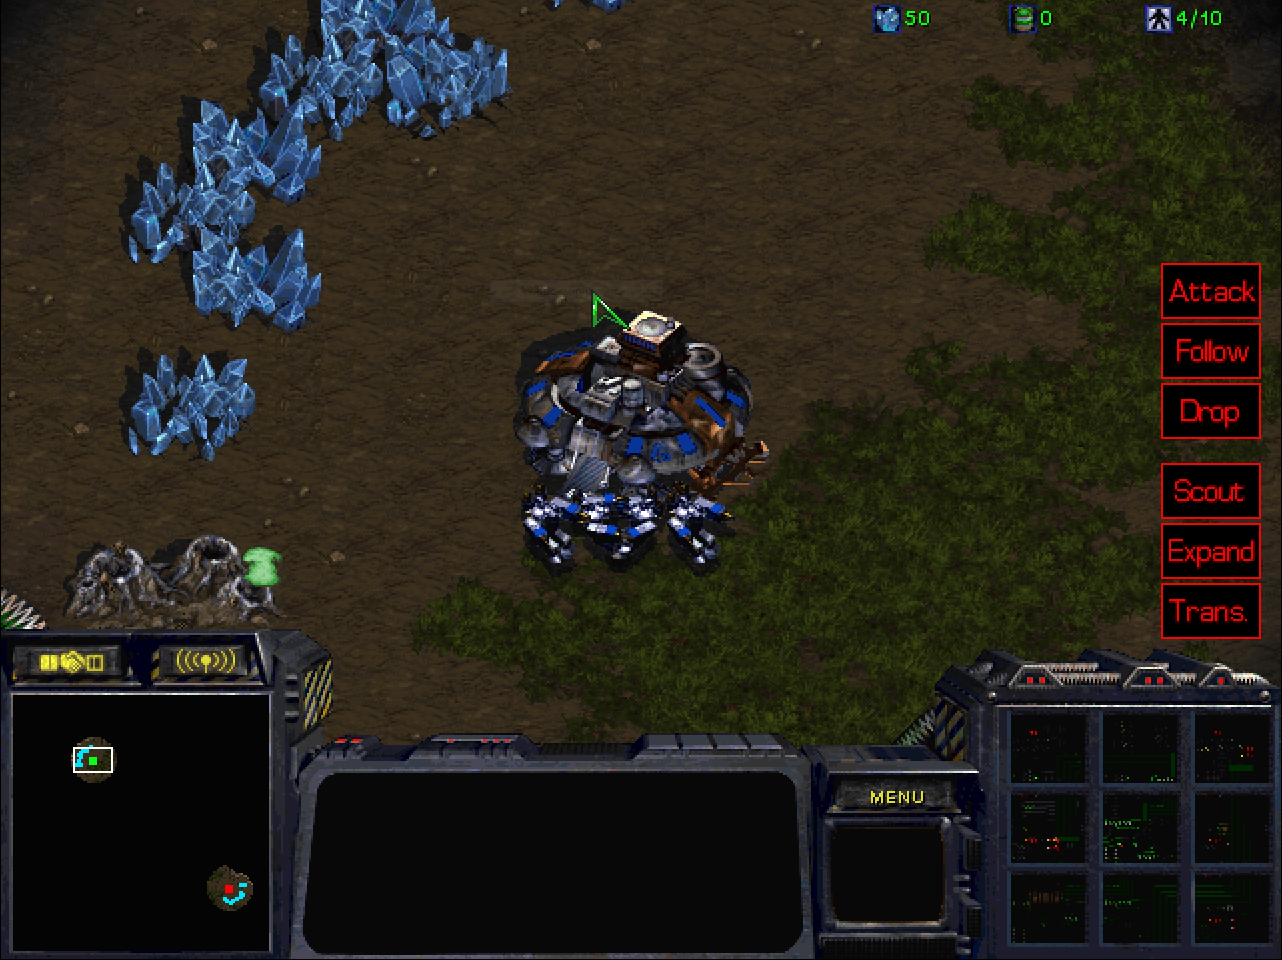
\includegraphics[width=0.8\textwidth]{player_gui_controls}
\caption{Player client with GUI commands enabled}
\label{fig:player_commands_gui}
\end{figure}

\section{Experiment method}
The experiment is divided into three parts, first the tester preparation where the testers plays
skirmish matches against the default bot to refresh his/her skills or familiarize him-/herself with
StarCraft and the map the experiment will be conducted on. The testers started the preparation
from a couple of days before the experiment to the day of the experiment.

The second part is the actually experiment itself. Here we present the tester with four scenarios:
\begin{inparaenum}[1\upshape)]
	\item no control over the bot and the bot would not communicate its intentions;
	\item with control over bot, but no communication;
	\item with communication, but no control; and
	\item with both control and communication enabled.
\end{inparaenum}
To avoid testers preferring a scenario depending on the order, i.e. the results depending on the
order, all testers will play the scenarios in different orders. This will, however, have a side effect:
tester that start with both communication and control might be overwhelmed with both having a
teammate, check its messages, and be able to control it.

The scenarios are played at fastest game speed, both because normal speed is slow (the experiment
would be too long) and it is considered a standard to play at fastest game speed in the StarCraft
community. Each scenario is limited to 20 minutes—if matches were longer (an hour) the tester might
be bored very quickly and would have to sacrifice a long time of their day. If the tester is winning
after 20 minutes, the tester was asked if we should speed up the game or close it—the matches were
sped up to roughly 10 times faster speed (depending on computer speed), thus the game usually ended
within a minute or two. This was done to let the player win for the experiment to continue to be
interesting.

\paragraph{Tester base}
The testers were all friends of us. The reasons we choose friends over strangers were:
\begin{inparaenum}[1\upshape)]
	\item we needed two computers as there is a bug that does not let you run the game on one computer
		unless you have installed a virtual machine;
	\item the testers should be comfortable when playing, thus we tested the game at their homes where
		we also got the second computer;
	\item the test was quite long, 1–3 hours of preparation and 2 hours in the experiment—we think it
		would be hard to get enough unknown players to be willing to play so long unless they were given
		some thanks money.
	\item we did not live near campus (2.5 hours and 5 hours away) meaning it would be quite expensive
		to commute or burdensome to stay at friends' places for a week to test on students.
\end{inparaenum}

Although we were aware of possible negative effects such as their answers being biased on what we
wanted to hear, we did not think this was enough to invalidate them as a tester base. All the 4
scenarios included our bot, meaning they would not test against another bot. They did not know our
thoughts or hypothesis before the experiment began and we tried to be as natural as possible not to
mention our thoughts.

\paragraph{Gathering results}
Directly after the 4 scenarios the tester was given a questionnaire asking to grade how fun each
scenario was in a scale from 1 (not fun) to 6 (very fun). The result from the questionnaire is
evaluated using paired two-sample T-tests.

Instead of testing whether the player thinks a scenario is fun or boring, we could test if s/he wins
or losses as one might think that winning is better than having fun. But the games we talk about is
for having fun and that does not mean winning, as only winning is actually quite
boring\cite{hagelback09}, and it is more fun to play when the player is challenges to play at his
best\cite{sweetser05}. \\

After the questionnaire the testers were interviewed using a semi-structured interview method. The
goal of this interview was to identify why they thought a scenario was more fun than the others,
what they liked, disliked, and missed about the bot.

\paragraph{Bot evaluation questions}
These are the main questions we wanted to answer during the interview.
\begin{compactitem}
	\item Which scenario did you think was most fun?
	\item What did you like most with the bot?
	\item What did you dislike?
	\item What did you miss?
	\item What command did you like?
	\item What command did you dislike?
	\item What command did you miss?
	\item When (if) you lost, did you feel it was the bot's fault, your own, or both?
	\item When (if) you won, did you feel it was because of the bot, you, or both?
	\item Was there anything that surprised you?
	\item Other comments?
\end{compactitem}

\paragraph{Experiment evaluation questions}
Some questions were asked about the experiment to get an overview how the testers perceived the
experiment to be, and possible improvements for the next experiment.
\begin{compactitem}
	\item	Was the experiment fun?
	\item Was the experiment too long?
	\item What did you think of the preparation? I.e. playing SC before the actual experiment.
	\item What improvements could be made to the experiment?
\end{compactitem}
